\section{影像检索}
\subsection{检索原则}
\begin{frame}
    根据人工的难易程度, 按照时间, 质量, 位置, 依次筛选数据
    \begin{itemize}
        \item 时间: 考虑正负14天的数据
        \item 质量: 考虑制作数据集成本, 云雾覆盖率, 云雾分布等情况筛选
        \item 位置: 哨兵大, 高分小. 保证边界盒有交集
    \end{itemize}
    
    \textbf{实际操作中, 先对哨兵数据和高分数据时间质量两者做筛选. 在筛选后的优质数据中, 寻找时间空间位置的交集.}
\end{frame}

\subsection{哨兵数据}
\begin{frame}{数据查询}
    \begin{columns}
        \column{0.3\textwidth}
        \begin{itemize}
            \item \small{对广东区域进行影像检索}
        \end{itemize}

        \column{0.7\textwidth}
        \begin{figure}
            \centering
            % Requires \usepackage{graphicx}
            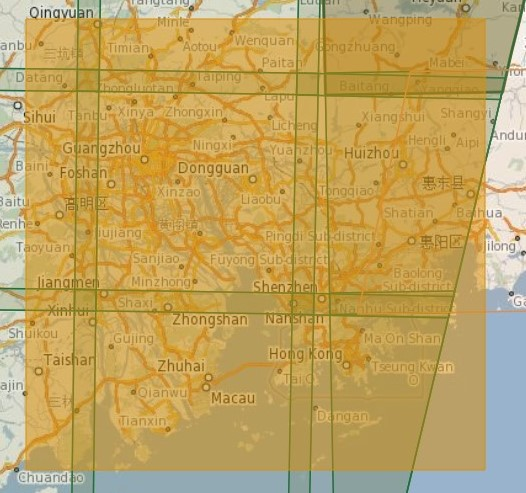
\includegraphics[width=5cm]{pic/pic0101.jpg}
            \caption{影像查询地区}
            \label{fig:0101}
        \end{figure}
    \end{columns}
\end{frame}

\begin{frame}{数据查询}
    \small{影像查询结果 $\frac{275}{2608} \approx 10.5\%$}, 在此中继续筛选, 可用数据为 $\frac{65}{2608} \approx 2.5\% $
    \begin{figure}[!htbp]
        \centering
        \subfloat[\tiny 全年数据]{\label{fig:0102a}
        
\includegraphics[height=4cm]{pic/pic0102.jpg}}
        \quad
        \subfloat[\tiny 云雾覆盖较少数据]{\label{fig:0102b}
        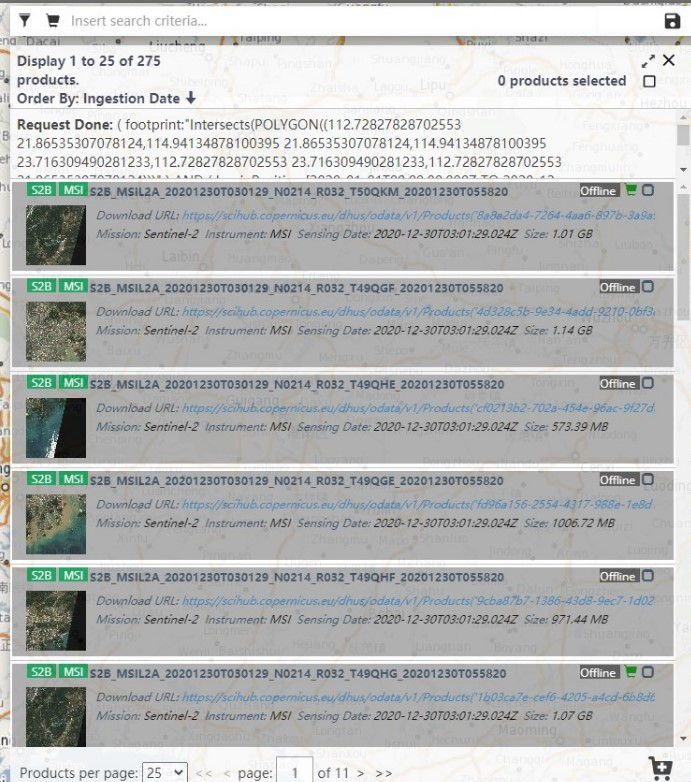
\includegraphics[height=4cm]{pic/pic0103.jpg}}
        \caption{2020-哨兵广东数据}
        \label{fig:0102}
    \end{figure}
\end{frame}

\begin{frame}{夏季数据不可用}
    \small{夏天数据整体云雾覆盖严重, 以5月6月数据为例}
    \begin{figure}[!htbp]
        \centering
        \subfloat[\tiny 5月数据]{\label{fig:0103a}
        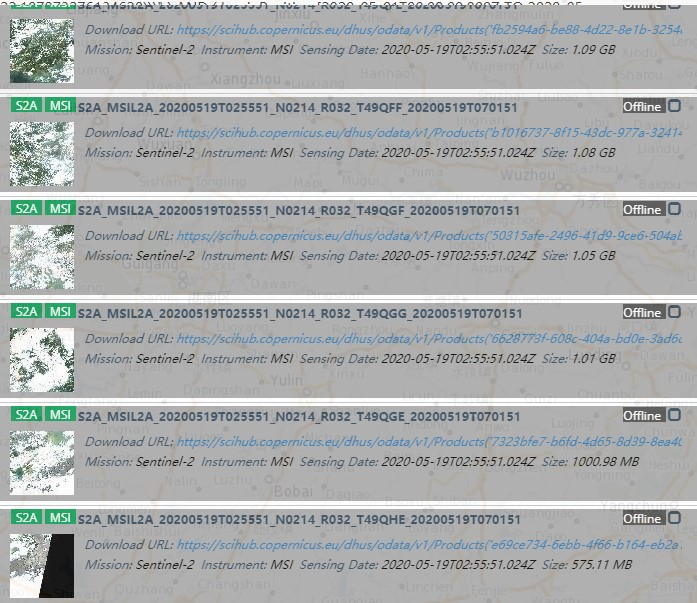
\includegraphics[width=4cm]{pic/pic0104.jpg}}
        \quad
        \subfloat[\tiny 6月数据]{\label{fig:0103b}
        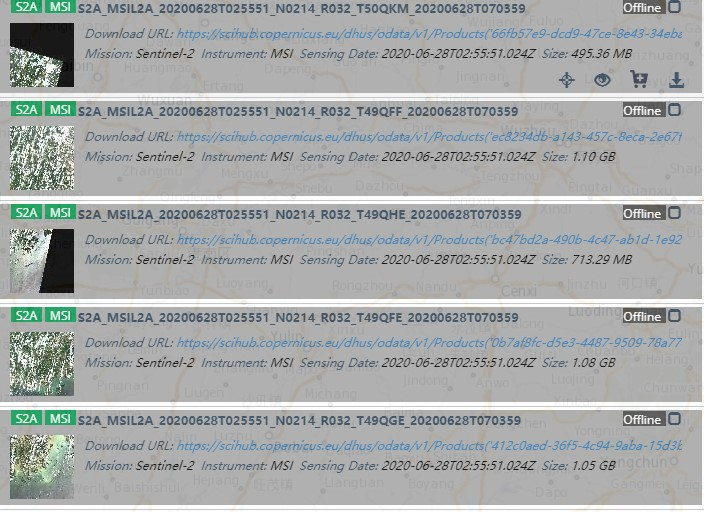
\includegraphics[width=4cm]{pic/pic0105.jpg}}
        \caption{5月6月数据}
        \label{fig:0103}
    \end{figure}
\end{frame}

\begin{frame}{不可用数据}
    \small{以下为质量过低而不可接受的数据}:
    \begin{figure}[!htbp]
        \centering
        \subfloat[\tiny 云覆盖严重]{\label{fig:0104a}
        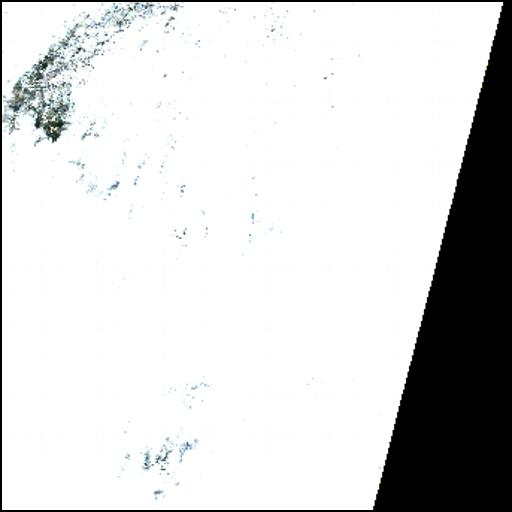
\includegraphics[width=4cm]{pic/pic0106.jpg}}
        \quad
        \subfloat[\tiny 可用数据过少]{\label{fig:0104b}
        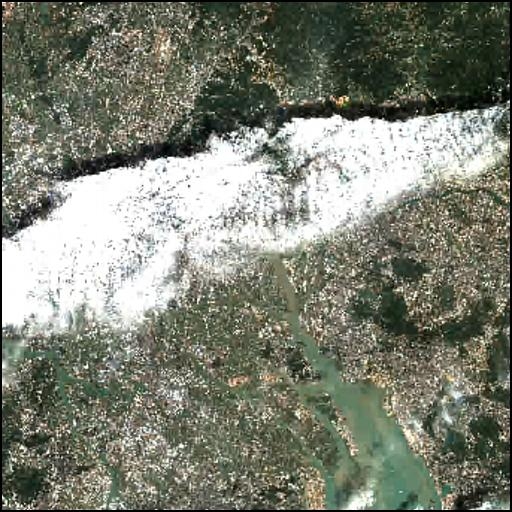
\includegraphics[width=4cm]{pic/pic0107.jpg}}
        \caption{云雾遮挡严重}
        \label{fig:0104}
    \end{figure}  
\end{frame}

\begin{frame}{可用数据}
    \small{除了完全无云雾的影像, 云雾分布集中一侧的也可使用}:
    \begin{figure}[!htbp]
        \centering
        \subfloat[\tiny 偏左下角]{\label{fig:0105a}
        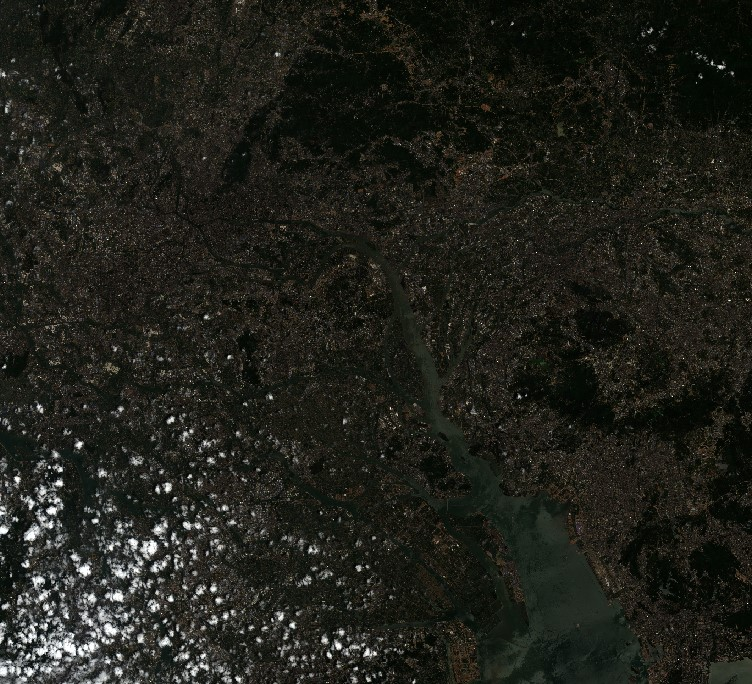
\includegraphics[width=4cm]{pic/pic0108.jpg}}
        \quad
        \subfloat[\tiny 偏左侧]{\label{fig:0105b}
        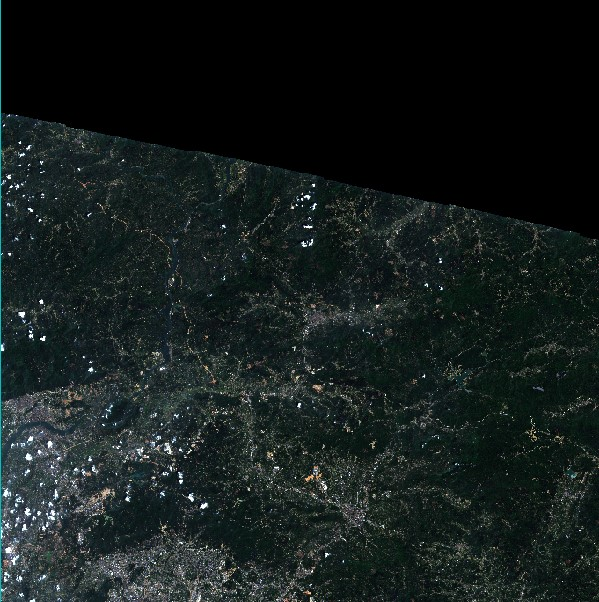
\includegraphics[width=4cm]{pic/pic0109.jpg}}
        \caption{可接受数据}
        \label{fig:0105}
    \end{figure}  
\end{frame}



\begin{frame}{检索结果}
    \small 
    可用数据有以下:
    \begin{itemize}
        \item 一月: 0115, 0130
        \item 二月: 0221
        \item 三月: 0315
        \item 四月: 0409, 0429
        \item 十月: 1011, 1026
        \item 十一月: 1105, 1125, 1130
        \item 十二月: 1205, 1227, 1230
    \end{itemize}
\end{frame}

\subsection{高分数据}
\begin{frame}{数据来源}
    由广东测绘院提供的高分辨率数据中包含很多卫星数据, 其区域都在广东省:
    \begin{itemize}
        \item 北京2
        \item GE1
        \item 高分1, 高分1B, 高分1C, 高分1D
        \item 高分2
        \item 高分6
        \item JL1
        \item WV2, WV3
        \item 资源3-1, 资源3-2
    \end{itemize}
\end{frame}

\begin{frame}{数据分布}
    维度范围: 21.9 -- 24.5, 经度范围: 112.2 -- 113.8
    \begin{figure}
        \centering
        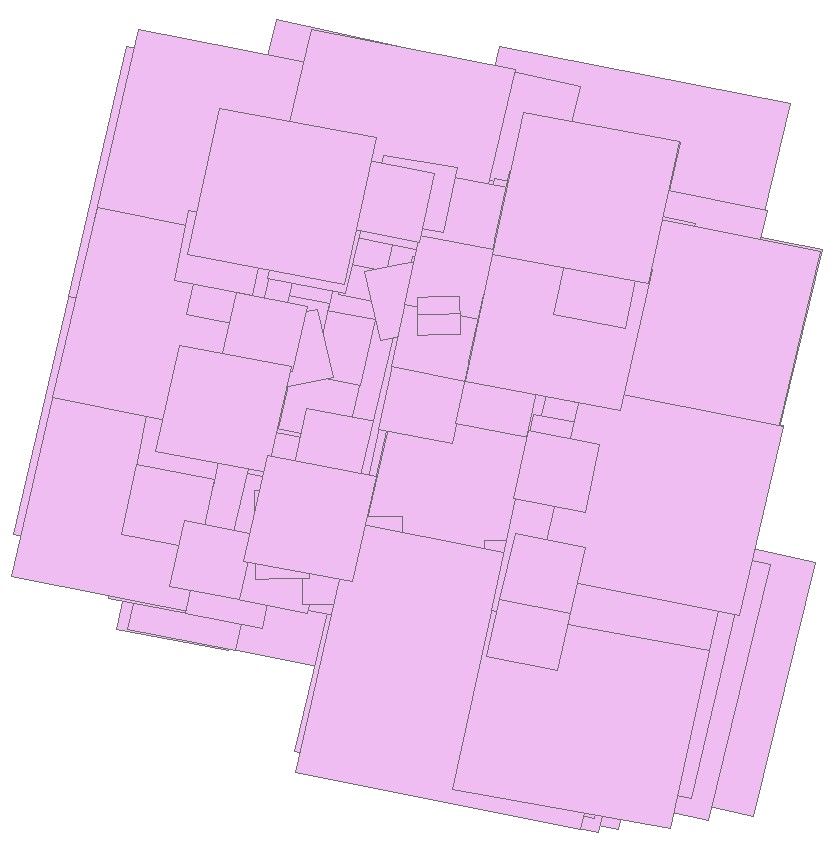
\includegraphics[width=5cm]{pic/pic0110.jpg}
        \caption{高分辨率整体}
        \label{fig:0106}
    \end{figure}
\end{frame}

\begin{frame}{数据分布属性表}
    在shp文件的属性表
    \begin{figure}
        \centering
        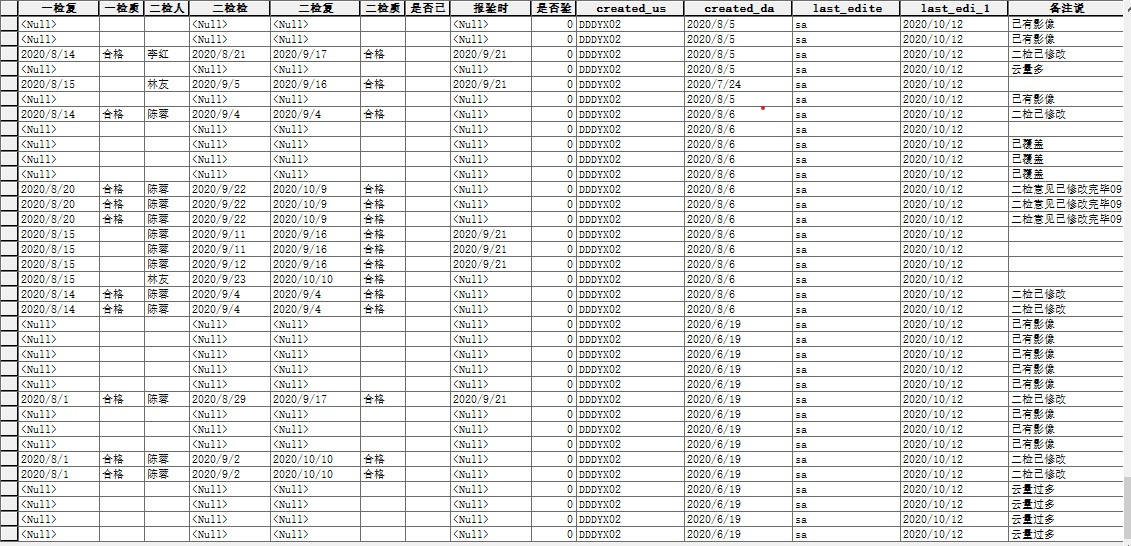
\includegraphics[width=8cm]{pic/pic0111.jpg}
        \caption{属性表}
        \label{fig:0107}
    \end{figure}
\end{frame}

\begin{frame}{高分时间筛选}
    针对高分一号, 高分二号数据进行筛选. 
    
    高分数据时间范围: 2019年12月至2020年7月
    
    排除无可用哨兵影像的5月-9月

    高分数据只需对2019年12月至2020年4月五个月数据进行查看

    由于高分数据被压缩两次, 解压时间成本较高

\end{frame}

\begin{frame}{高分质量筛选}
    除去云雾覆盖较为严重的影像:
    \small{除了完全无云雾的影像, 云雾分布集中一侧的也可使用}:
    \begin{figure}[!htbp]
        \centering
        \subfloat[\tiny 云雾覆盖]{\label{fig:0108a}
        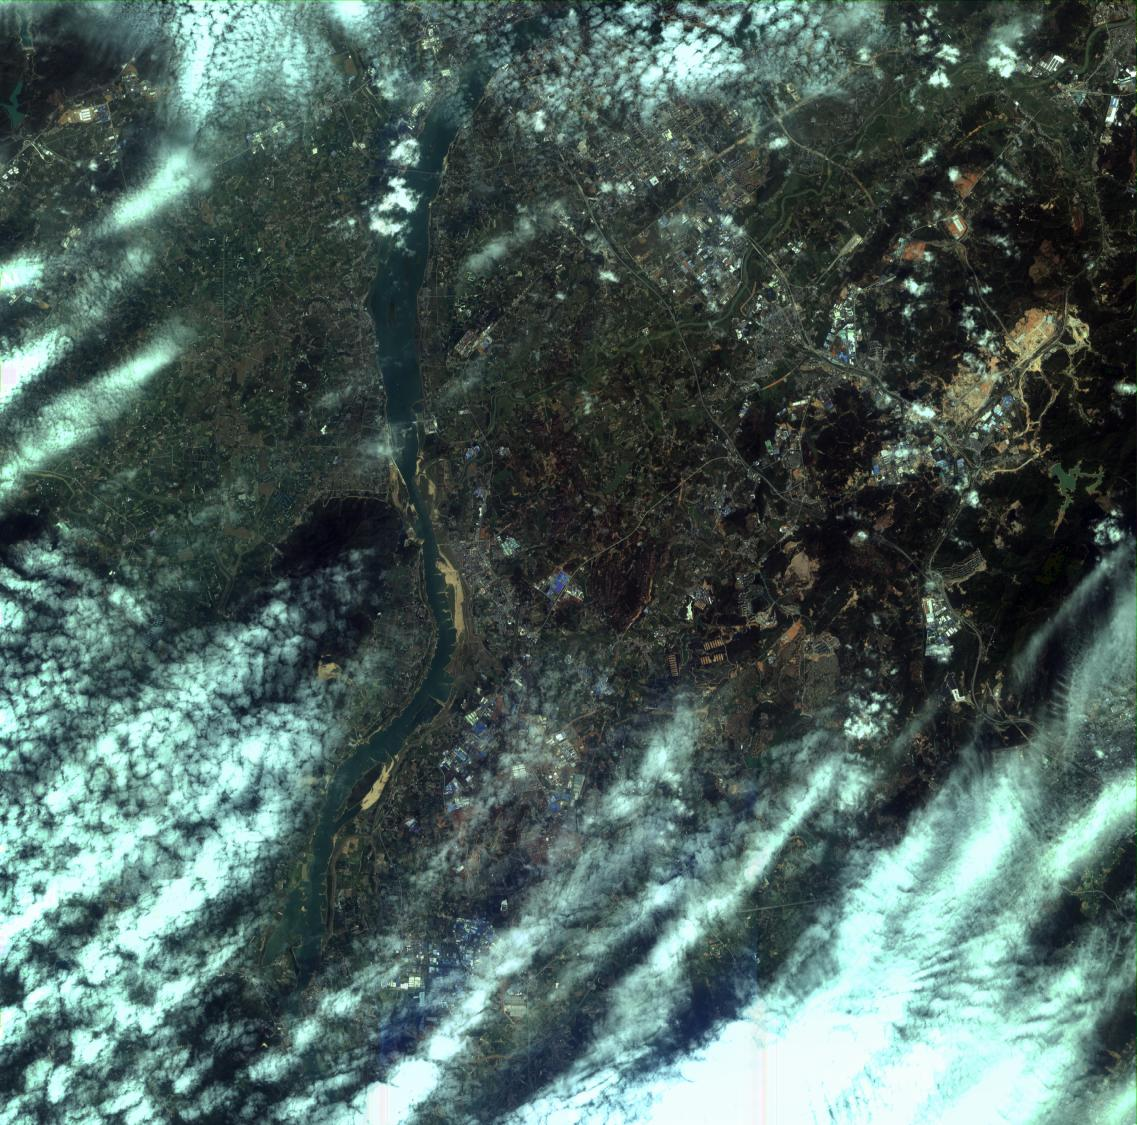
\includegraphics[width=4cm]{pic/pic0112.jpg}}
        \quad
        \subfloat[\tiny 云雾覆盖]{\label{fig:0108b}
        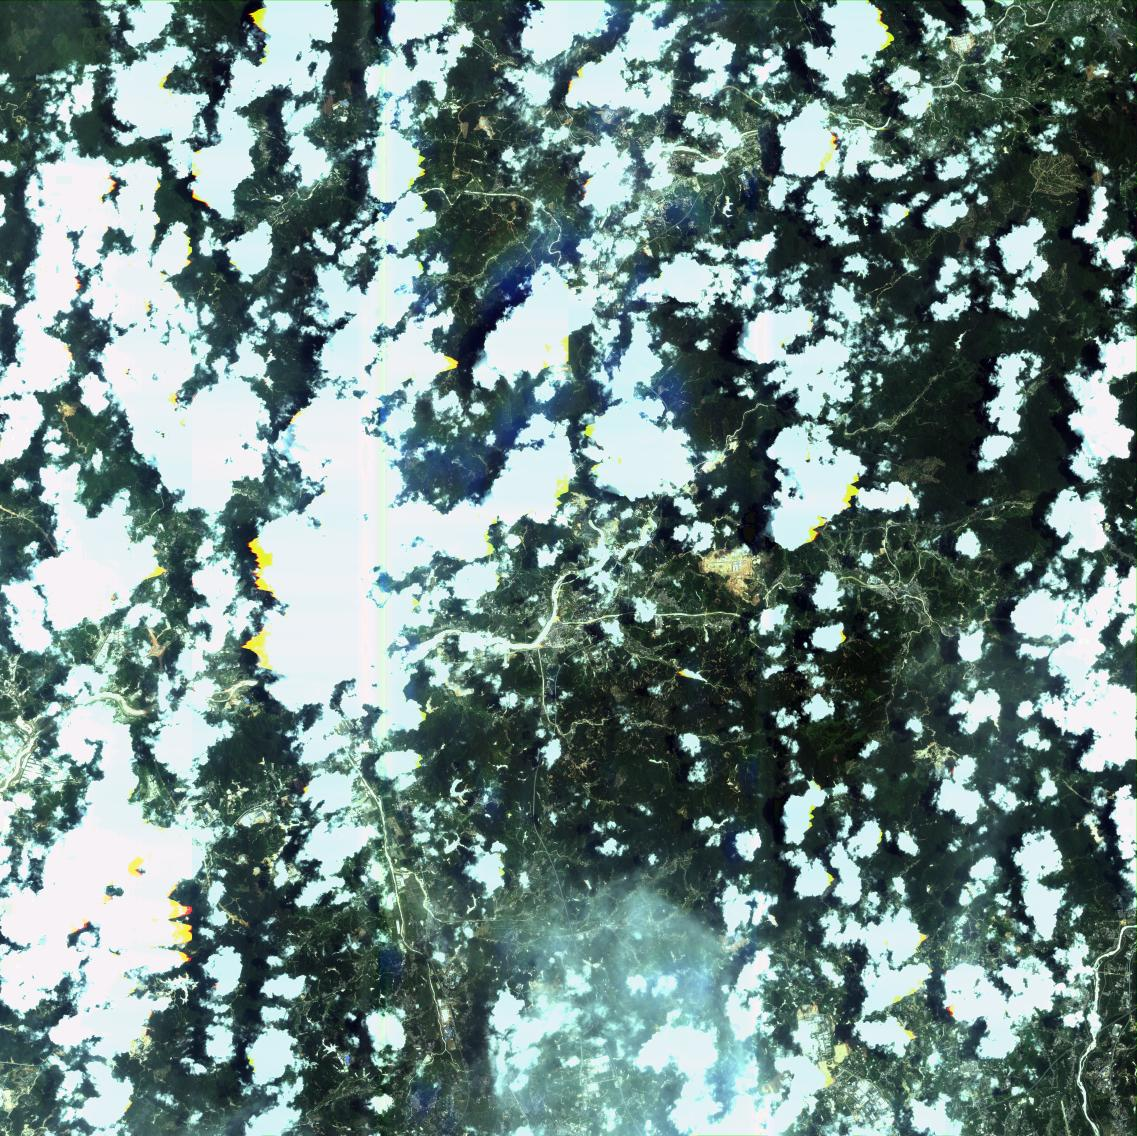
\includegraphics[width=4cm]{pic/pic0113.jpg}}
        \caption{云雾覆盖严重}
        \label{fig:0108}
    \end{figure}
\end{frame}

\begin{frame}{高分可用数据}
    其数据为:
    \tiny
    \begin{itemize}
        \item E112.8N22.720200314L1A0004699153
        \item E112.8N23.020200314L1A0004699151
        \item E112.9N23.320200314L1A0004699152
        \item E113.3N22.720200129L1A0004585377
        \item E113.4N23.020200129L1A0004585375
        \item E113.4N23.320200129L1A0004585374
        \item E113.5N23.620200129L1A0004585373
        \item E113.2N22.920200314L1A0004838272
        \item E113.2N23.220200314L1A0004824312
        \item E113.3N23.520200314L1A0004824311
        \item E113.4N23.820200314L1A0004672017
        \item E113.8N23.220200129L1A0004585596
        \item E113.8N23.520200129L1A0004585595
        \item E113.9N22.920200412L1A0004736006
        \item E113.9N23.820200129L1A0004585594
        \item E114.0N23.220200412L1A0004736005
        \item E114.1N23.820200412L1A0004736003
    \end{itemize}
\end{frame}

\begin{frame}{高分可用数据}
    所找到可用高分影像如图所示:
    \begin{figure}
        \centering
        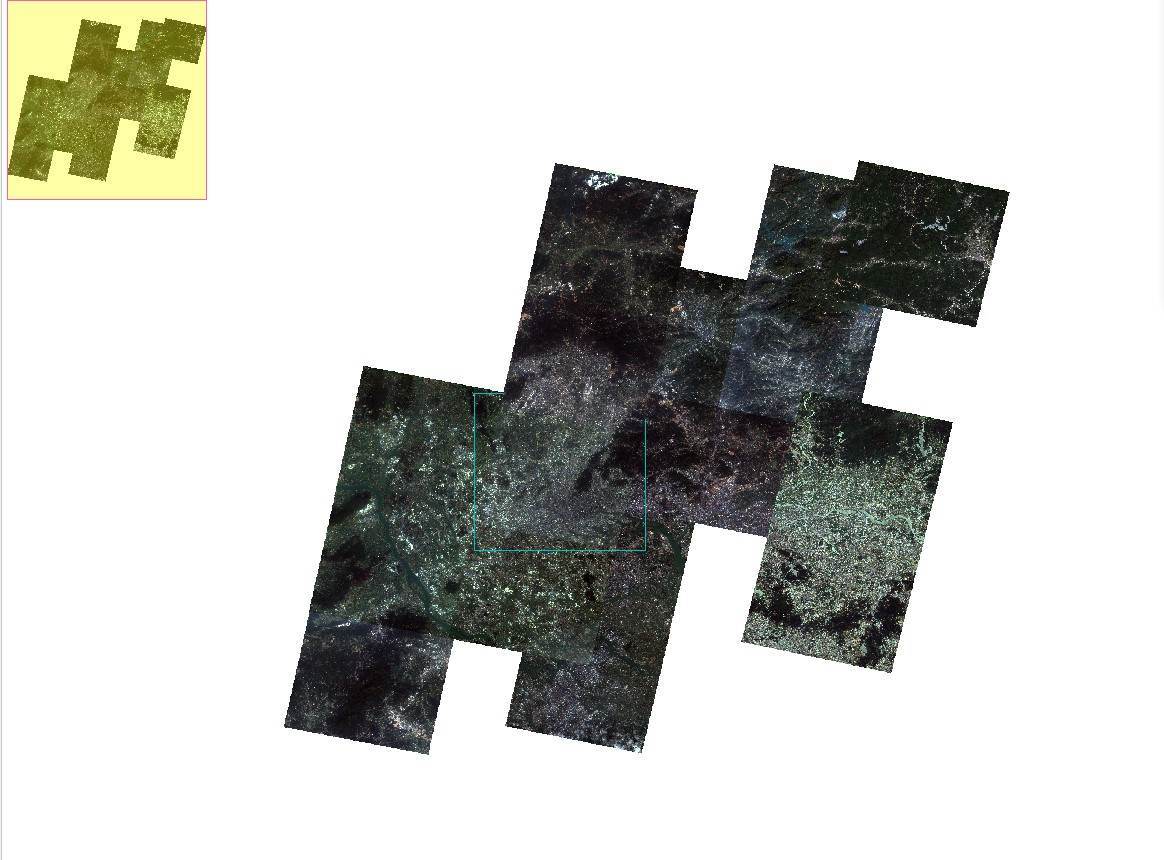
\includegraphics[width=7cm]{pic/pic0114.jpg}
        \caption{高分可用数据}
        \label{fig:0109}
    \end{figure}
\end{frame}

\subsection{数据交集}
\begin{frame}{空间交集}
    筛选高分数据时, 已经使用了哨兵数据的时间信息

    现在只做空间交集

    发现高分0314数据与哨兵0315数据在空间上没有重叠

    因此剔除该数据, 得到三个子数据集
\end{frame}

\begin{frame}{可用哨兵数据列表}
    \small
    以下为可用哨兵数据列表:
    \begin{itemize}
        \item 20200130T025941\_N0213\_R032\_T49QGG 
        \item 20200130T025941\_N0213\_R032\_T49QGF
        \item 20200429T025551\_N0214\_R032\_T49QGF
        \item 20200429T025551\_N0214\_R032\_T49QGG
        \item 20200429T025551\_N0214\_R032\_T50QKM
        \item 20191226T030129\_N0213\_R032\_T49QGF
    \end{itemize}
\end{frame}

\begin{frame}{2019-12-27子数据集}
    \small 哨兵数据为
    \tiny
    \begin{itemize}
        \item 20191226T030129N0213R032T49QGF
    \end{itemize}
    \small 高分数据为
    \tiny
    \begin{itemize}
        \item E113.1N22.820191227L1A0004731172
        \item E113.1N23.020191227L1A0004507320
        \item E113.2N23.320191227L1A0004507303
        \item E113.3N22.820191227L1A0004505423
        \item E113.3N22.920191227L1A0004505422
        \item E113.4N23.120191227L1A0004505416
    \end{itemize}
\end{frame}

\begin{frame}{2020-01-29子数据集}
    \small 哨兵数据为
    \tiny
    \begin{itemize}
        \item 20200130T025941N0213R032T49QGG
        \item 20200130T025941N0213R032T49QGF
    \end{itemize}
    \small 高分数据为
    \tiny
    \begin{itemize}
        \item E113.3N22.720200129L1A0004585377
        \item E113.4N23.020200129L1A0004585375
        \item E113.4N23.320200129L1A0004585374
        \item E113.5N23.620200129L1A0004585373
        \item E113.8N23.220200129L1A0004585596 上半幅
        \item E113.8N23.520200129L1A0004585595 要匹配两次, 横跨哨兵上下两幅
        \item E113.9N23.820200129L1A0004585594
    \end{itemize}
\end{frame}

\begin{frame}{2020-04-29子数据集}
    \begin{columns}
        \column{0.5\textwidth}
        \small 哨兵数据为
        \tiny
        \begin{itemize}
            \item 20200429T025551N0214R032T49QGF
            \item 20200429T025551N0214R032T49QGG
            \item 20200429T025551N0214R032T49QKM
        \end{itemize}
        \small 高分数据为
        \tiny
        \begin{itemize}
            \item E113.9N22.920200412L1A0004736006
            \item E114.0N23.220200412L1A0004736005
            \item E114.1N23.820200412L1A0004736003
        \end{itemize}

        \column{0.5\textwidth}
        \tiny
        \begin{itemize}
            \item E113.8N23.120200428L1A0004767988
            \item E113.8N23.320200428L1A0004767982
            \item E113.9N23.520200428L1A0004767976
            \item E113.9N23.720200428L1A0004768005
            \item E114.0N23.920200428L1A0004768001
            \item E113.9N22.820200428L1A0004768660
            \item E114.2N23.820200428L1A0004768656
        \end{itemize}
    \end{columns}
\end{frame}

\begin{frame}{可用哨兵数据空间位置}
    \small
    考虑到六幅影像的范围有重叠, 只用其中一组即可
    \begin{figure}
        \centering
        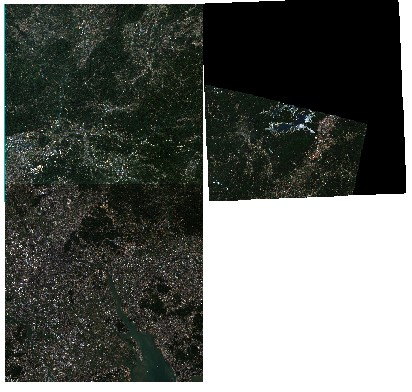
\includegraphics[width=6cm]{pic/pic0115.jpg}
        \caption{哨兵可用重叠}
        \label{fig:0109}
    \end{figure}
\end{frame}